% Modelo de Avaliação em LaTeX
% IFPR - Paranavaí
% Se utilizar o Overleaf, clique em RICH TEXT acima para uma visualização mais suave do código!
% Edição para CEFET-RJ: Haron Calegari Fanticelli

\documentclass[a4paper,11pt]{article}

%-------------------------------------------------------------------------
% PACOTES (não é necessário alterar nada) 
%-------------------------------------------------------------------------

\usepackage[utf8]{inputenc}
\usepackage[brazil]{babel} 
\usepackage{graphicx}
\usepackage{color} 
\usepackage{hyperref} 
\usepackage{geometry} 
\usepackage{amsmath,amsthm,amsfonts,amssymb,amscd,amsxtra} 
\usepackage{multicol}
\usepackage{multirow}
\usepackage{enumerate}
\usepackage{tikz}
\usetikzlibrary{positioning,shapes,fit,arrows,through,calc,shapes.geometric,patterns,decorations.markings}
\usepackage{pgf,pgfplots}
\usepgfplotslibrary{fillbetween}
\pgfplotsset{compat=1.15}
\usepackage{mathrsfs}
\definecolor{myblue}{RGB}{56,94,141}
\definecolor{mygreen}{RGB}{51,153,0}
\definecolor{myred}{RGB}{204,0,0}
\usepackage{setspace}
\geometry{a4paper,left=1.5cm,right=1.5cm,top=1.5cm,bottom=1.5cm}

\usepackage{comment}
\usepackage{subfigure}
\usepackage{minted}

%-------------------------------------------------------------------------
% INFORMAÇÕES DA AVALIAÇÃO (PREENCHA)
%-------------------------------------------------------------------------

\newcommand{\professor}{Haron C. Fanticelli}
\newcommand{\disciplina}{Pesquisa Operacional I}
\newcommand{\trimestre}{6º}
\newcommand{\curso}{Engenharia de Produção}
\newcommand{\turno}{}
\newcommand{\instrumento}{Exercícios (p/ Casa)} % Pode ser Prova Escrita, Trabalho em classe, Trabalho Extraclasse, Relatório, etc.

%-------------------------------------------------------------------------
% CABEÇALHO (não é necessário alterar nada) 
%-------------------------------------------------------------------------

\begin{document}

\pagestyle{empty}

\begin{minipage}{6cm} %Logo do CEFET

\includegraphics[scale=.8, trim={0.5cm 0.5cm 0.5cm 0.5cm}, clip]{horiz_azul_itaguai.png}
\end{minipage}
\begin{minipage}{7cm}
\begin{center}
\begin{footnotesize}
\sf \textbf{Centro Federal de Educação Tecnológica Celso Suckow da Fonseca}\\
\textbf{Uned Itaguaí}\\
%Rod. Gov. Mário Covas \\
%Santana - Itaguaí - RJ
\end{footnotesize}
\end{center}
\end{minipage}
\begin{minipage}{4cm}
\centering

\includegraphics[scale=0.12]{meBrasil.png}\\
\begin{scriptsize}
\textsf{Ministério da Educação}
\end{scriptsize}
\end{minipage}
\doublespacing
\begin{center}
\begin{tabular}{|l|l|l|}
\hline
\textbf{Curso:} \curso & \textbf{Turno:} \turno & \textbf{Período:} \trimestre \\
\hline
\multicolumn{2}{|l|}{\textbf{Disciplina:} \disciplina} & \textbf{Professor(a):} \professor  \\
\hline
\multicolumn{2}{|l|}{\textbf{Nome:}} & \textbf{Valor:} -- pontos \\
\hline
\textbf{Nota:}  & \textbf{\instrumento} & \textbf{Data:} 09/2023  \\
\hline
\end{tabular}
\end{center}
\singlespacing

%-------------------------------------------------------------------------
% EXPECTATIVAS DE APRENDIZAGEM 
%-------------------------------------------------------------------------

%-------------------------------------------------------------------------
% QUESTÕES ou ENUNCIADOS
%-------------------------------------------------------------------------
\vspace{-.2cm}

\begin{enumerate}
    \item Um certo modelo de programação linear envolvendo duas atividades possui a região de soluções viáveis indicada a seguir:
    
    \begin{figure}[H]
        \centering
        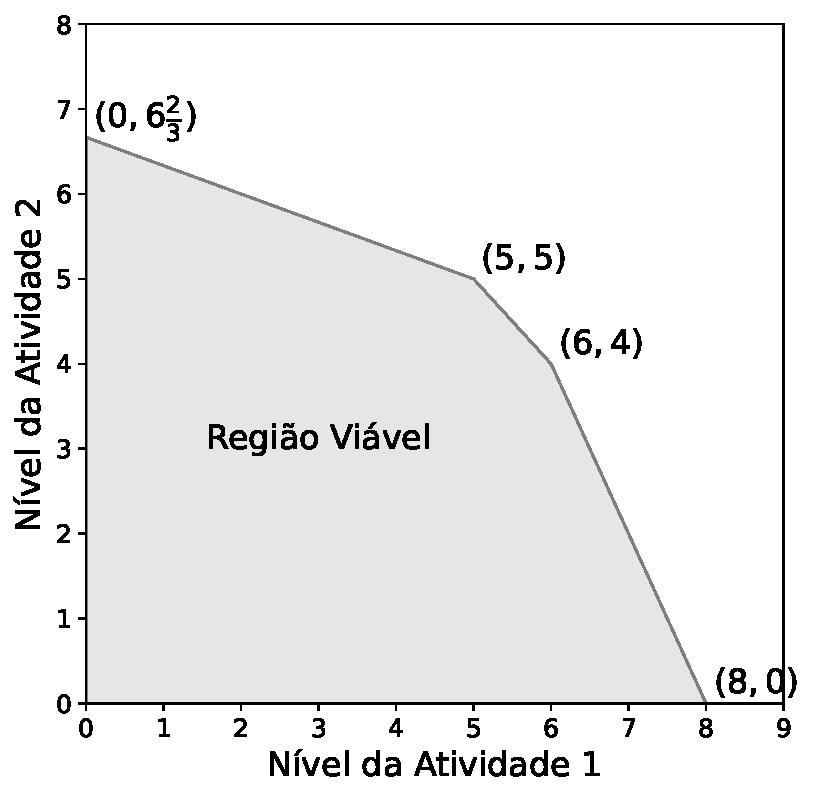
\includegraphics[scale=.45]{images/exerc_4.1-3.pdf}
    \end{figure}

    O objetivo é maximizar o lucro total das duas atividades. O lucro unitário para a atividade 1 é de US\$ 1.000 e o lucro unitário para a atividade 2 é de US\$ 2.000.
    \begin{enumerate}
        \item Calcule o lucro total para cada solução de pontos extremos. Use esta informação para encontrar uma solução ótima.
        \item Use os conceitos de solução do Método Simplex para identificar a sequência de soluções que seriam examinados pelo método até chegar a solução ótima.
    \end{enumerate}




    \item Pelo método simplex, passo a passo, solucione o problema a seguir:
    \begin{align*}
        \begin{matrix}
            \text{Maximizar} & Z = 4x_1 + 3x_2 + 6x_3 \\
            \text{Sujeito a} & 3x_1 + x_2 + 3x_3 \leq 30 \\
                             & 2x_1 + 2x_2 + 3x_3 \leq 40 \\
            \text{e}         & x_1 \geq 0 \text{, } x_2 \geq 0 \text{, } x_3 \geq 0
        \end{matrix}
    \end{align*}





    \item Descreva graficamente o que o método simplex faz passo a passo para solucionar o problema a seguir:
    \begin{align*}
        \begin{matrix}
            \text{Maximizar} & Z = 2x_1 + 3x_2 \\
            \text{Sujeito a} & -3x_1 + x_2 \leq 1 \\
                             & 4x_1 + 2x_2 \leq 20 \\
                             & 4x_1 - x_2 \leq 10 \\
                             & -x_1 + 2x_2 \leq 5 \\
            \text{e}         & x_1 \geq 0 \text{, } x_2 \geq 0
        \end{matrix}
    \end{align*}
\end{enumerate}

\end{document}